\newcommand{\R}{\mathbb{R}}
\newcommand{\M}{\mathbb{M}}
\newcommand{\syst}[2]{\left\{ \begin{array}{#1} #2 \end{array} \right.}
\newcommand{\trans}{\mathsf{T}}
\newcommand{\ind}{\mathbbm{1}}

\definecolor{darkWhite}{rgb}{0.94,0.94,0.94}
\definecolor{whiteGray}{rgb}{0.8,0.82,0.8}
\definecolor{blue}{rgb}{0.12,0.16,0.53}
\definecolor{green}{rgb}{0.25,0.28,0.06}
\definecolor{greenTikz}{rgb}{0.16,0.53,0.12}
\definecolor{red}{rgb}{0.71,0.19,0.11}

\chapauthor{Yoann Coudert--Osmont}

\motto{
	Ce chapitre a pour but d'étendre à des variétés, certaines opérations statistiques usuellement réalisés sur des espaces euclidiens.
}

\chapter{Moyenne, variance et régression géodésique}
\label{chap:stats}

\section{Régression géodésique}
\label{sec:Regression}

\subsection{Rappel : Régression linéaire}
\label{subsec:RegLin}

Dans le cas d'une régression linéaire classique, on se donne un jeu de données $\{ y_i, t_i \}_{i = 1, ..., N}$ avec $y_i \in \R^n$ et $t_i \in \R_+$. On souhaite alors expliquer les données par une fonction affine paramétré par les vecteurs $\alpha$ et $\beta$ dans $\R^n$ :
\begin{equation}
	\label{eq:RegLin}
	y_i = \gamma(t_i) + \epsilon_i \qquad \text{avec} \quad \gamma(t) = \alpha t + \beta
\end{equation}
L'objectif est alors de trouver des paramètres qui minimisent les $\epsilon_i$. On minimise généralement la somme des carrés de leur norme :
\begin{equation}
	E(\alpha, \beta) = \sum_{i=1}^N \| \epsilon_i \|^2 = \sum_{i=1}^N \| \gamma(t_i) - y_i \|^2
\end{equation}

\begin{figure}[t]
	\centering
	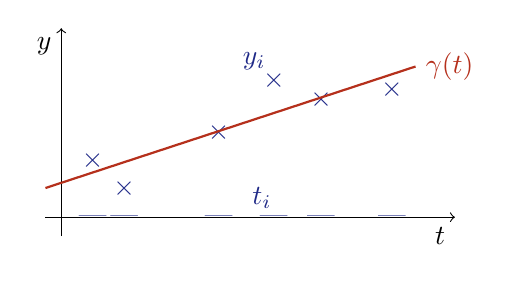
\begin{tikzpicture}[yscale=1.2]
		\draw[->] (-0.2, 0) -- (5, 0) node[below left] {$t$}; 
		\draw[->] (0, -0.2) -- (0, 2) node[below left] {$y$};
		
		\node[blue] at (0.4, 0) {|};
		\node[blue] at (0.8, 0) {|};
		\node[blue] at (2.0, 0) {|};
		\node[blue] at (2.7, 0) {|};
		\node[blue] at (3.3, 0) {|};
		\node[blue] at (4.2, 0) {|};
		\node[blue] at (0.4, 0.60) {$\times$};
		\node[blue] at (0.8, 0.30) {$\times$};
		\node[blue] at (2.0, 0.90) {$\times$};
		\node[blue] at (2.7, 1.45) {$\times$};
		\node[blue] at (3.3, 1.25) {$\times$};
		\node[blue] at (4.2, 1.35) {$\times$};
		\node[blue] at (2.45, 1.65) {$y_i$};
		\node[blue] at (2.55, 0.2) {$t_i$};
		
		\draw[red, thick] (-0.2, 0.309) -- (4.5, 1.595) node[right] {$\gamma(t)$};
	\end{tikzpicture}
	\caption{Régression linéaire dans un espace euclidien.}
\end{figure}

\subsection{Régression sur une variété}
\label{subsec:RegGeo}

Désormais nos données $y_i$ ne vivent plus sur un espace euclidien $\R^n$ mais sur une variété $\M$. Les notions d'addition et de multiplication par un scalaire ne sont alors plus définis. On ne peut plus considérer de fonctions affines. Une solution envisageable est de prendre $\gamma$ dans l'ensemble des géodésiques. On peut justifier ce choix par le fait que les géodésiques dans les espaces euclidiens sont les fonction affines. On paramétrise alors $\gamma$ par $p_0 \in \M$ la position initiale à $t=0$ et $v_0 \in T_p \M$ la vitesse initiale. L'équation \eqref{eq:RegLin} devient donc :
\begin{equation}
	\gamma(t) = \Exp_{p_0} (t v_0)
\end{equation}
On minimise alors la distance entre les $y_i$ et les $\gamma(t_i)$ :
$$ E(p_0, v_0) = \sum_{i=1}^N D \left( y_i, \Exp_{p_0}(t_i v_0) \right) $$
Cette fonction de distance $D$ pourrait être la distance géodésique, mais elle est généralement compliqué à calculer. Si notre variété $\M$ est une sous-variété d'un espace euclidien alors on peut prendre la distance euclidienne au carré. Cette distance possède une moindre signification sur la variété mais elle a l'avantage d'être facilement calculable et différentiable.
$$ \text{exemple :} \quad D(x, y) = \| x - y \|^2 $$
On utilise ensuite un formalisme vu dans les chapitres précédents. On pose :
\begin{equation}
	S(t) = \pm{p(t) \\[1mm]\ q(t)} \qquad \text{avec } \syst{lll}{p(0) & = & p_0 \\[1mm] q(0) & = & g_{p_0} v_0}
\end{equation}
Puis on considère l'opérateur $F$ qui contrôle l'évolution de $S$ :
\begin{equation}
	\label{eq:op_F}
	F = \pm{\partial_q H \\[1mm] - \partial_p H} \qquad \text{avec } H(p, q) = \frac{1}{2} q^\trans g_p^{-1} q
\end{equation}
De sorte à avoir l'équation Hamiltonienne des géodésiques formulée via :
\begin{equation}
	\label{eq:evol_S}
	\syst{lll}{
		\dot{S}(t) = F(S(t)) \\[1mm]
		S(0) = S_0
	}
\end{equation}
On cherche alors à minimiser :
\begin{equation}
	E(S_0) = \sum_{i=1}^N f_i(S(t_i)) \qquad \text{avec } f_i(p, q) = D(y_i, p)
\end{equation}
Afin de pouvoir effectuer une descente de gradient pour trouver le paramètre $S_0$ qui minimise $E$, on s'intéresse à la variation de l'énergie $\delta E$, après une variation $\delta S_0$ des conditions initiales. A l'aide du système qui régi $S$ \eqref{eq:evol_S}, on déduit le système qui régi l'impact de la variation initiale $\delta S_0$ le long de $S$ :
\begin{equation}
\label{eq:evol_dS}
\syst{lll}{
	\dot{\delta S}(t) = d_{F(S(t))} \delta S(t) \\[1mm]
	\delta S(0) = \delta S_0
}
\end{equation}
En intégrant on obtient la variation de $S$ au temps $t$ :
\begin{equation}
	\label{eq:dS}
	\delta S(t) = \exp \left( \int_0^{t} \d_{S(u)} F du \right) \delta S_0
\end{equation}
Ce qui nous permet alors de calculer la variation de $E$ :
\begin{equation}
	\label{eq:deltaEreg}
	\delta E = \sum_{i=1}^N \d_{S(t_i)} f_i \delta S(t_i) = \sum_{i}^N \d_{S(t_i)} f_i \exp \left( \int_0^{t_i} \d_{S(u)} F du \right) \delta S_0
\end{equation}
On peut ensuite écrire le gradient de $E$ à partir de cette équation :
\begin{equation}
	\nabla_{S_0} E = \sum_{i=1}^N \exp \left( \int_0^{t_i} \d_{S(u)} F^\trans du \right) \nabla_{S(t_i)} f_i
\end{equation}
Afin de transformer le calcul de ce gradient en la résolution d'un système, on pose la fonction suivante :
\begin{equation}
	\nu(t) = \sum_{i=1}^N \exp \left( \int_t^{t_i} \d_{S(u)} F^\trans du \right) \nabla_{S(t_i)} f_i \ind \{ t \leqslant t_i \}
\end{equation}
On remarque alors l'égalité $\nabla_{S_0} E = \nu(0)$. Puis en dérivante cette fonction on aboutit à la proposition suivante.

\begin{proposition}
	Le gradient de $E$ est la solution à $t=0$ du système :
	\begin{equation}
		\syst{lll}{
			\dot{\nu}(t) & = & - d_{S(t)} F^\trans \nu(t) - \sum_{i=1}^N \nabla_{S(t_i)} f_i \delta (t - t_i) \\[1mm]
			\nu(T) & = & 0
		}
	\end{equation}
	Où $T > \sup_{i = 1}^N t_i$.
\end{proposition}

\begin{remarque}
	Dans le cas où $N=1$ et en fixant le point initial $p_0$, cette régression géodésique revient à calculer le log riemannien de $y_1$ depuis la position $p_0$, $\Log_{p_0}(y_1)$.
\end{remarque}

\begin{figure}[t]
	\centering
	\begin{tikzpicture}[scale=0.7]
		\shade[left color=darkWhite!90, right color=whiteGray!90] 
		(1.5,-2) to[out=15,in=170] (11.2,-1.8) node[above right] {\large $\M$} to[out=85, in=-70] (10.2,2.5) to[out=165,in=15] (1,2.2) -- cycle;
		
		\coordinate (p0) at (3.5, -0.5);
		\coordinate (p1) at (9.5, 1.5);
		
		\draw[red, thick] (p0) to[out=28, in=172] node[above] {$\gamma(t)$} coordinate[pos=0.12] (geo1) coordinate[pos=0.36] (geo2) coordinate[pos=0.58] (geo3) coordinate[pos=0.83] (geo4) (p1);
		\draw[->, >=angle 60, greenTikz, thick] (p0) -- node[below=1mm] {$\;v_0$} +(0.706, 0.376);
		
		\node[red] at (p0) {$\bullet$};
		\node[red, left] at (p0) {$p_0 = \gamma(0)$};
		\node[red] at (p1) {$\bullet$};
		\node[red, right] at (p1) {$\gamma(T)$};
		
		\coordinate (nu1) at (4,0.4);
		\coordinate (nu2) at (5,1.3);
		\coordinate (nu3) at (7.5,0.42);
		\coordinate (nu4) at (8.5,1.1);
		
		\draw[orange, dashed] (nu1) to (geo1);
		\draw[orange, dashed] (nu2) to[out=-40, in=120] (geo2);
		\draw[orange, dashed] (nu3) to[out=110, in=-40] (geo3);
		\draw[orange, dashed] (nu4) to (geo4);
		\draw[blue] (nu1) node {$\bullet$} node[above] {$y_1$};
		\draw[blue] (nu2) node {$\bullet$} node[above] {$y_2$};
		\draw[blue] (nu3) node {$\bullet$} node[below] {$y_3$};
		\draw[blue] (nu4) node {$\bullet$} node[below] {$y_4$};
	\end{tikzpicture}
	\caption{Régression géodésique sur une variété.}
\end{figure}

\subsection{Régression sur une variété morphométrique}

\paragraph{Définition du problème}
Désormais on s'intéresse à la déformation d'une forme au cours du temps. On se donne toujours des temps $t_i \geqslant 0$ associés à des formes $y_i \in \M = \R^{dM}$, représentés par des $M$-uplets de point dans un espace de dimension $d$. On se donne ensuite une forme initiale au temps $t = 0$ que l'on note $X_0$, puis on cherchera à calculer une évolution temporelle de cette forme $X(t)$ avec $X(0) = X_0$ qui soit suffisamment proche des $y_i$ aux temps $t_i$. On minimisera donc l'énergie :
\begin{equation}
	\label{eq:E_morph}
	E(X_0, S_0) = \sum_{i=1}^N D(X(t_i), y_i) = \sum_{i=1}^N f_i(X(t_i))
\end{equation}
Où comme précédemment la distance $D$ est usuellement la distance euclidienne, et $S_0$ est un ensemble de paramètres initiaux contrôlant l'évolution de $X$. Il nous faut alors paramétriser notre fonction $X$ et ainsi déterminer $S_0$. Pour cela, on se donne un RKHS $V$ de champs de vecteurs sur $\R^d$ muni du noyau $K$. Ce RKHS engendre un groupe de difféomorphisme $\mathcal{G}_V$. Ce sont ces difféomorphismes qu'on utilisera pour déformer $X_0$. Mais pour cela il nous faut un champs de vecteur de $V$ qui évolue au cours du temps. Grâce au noyau on peut représenter ce champs via des points de contrôle $c_i \in \R^d$ auxquels on associe des moments $\alpha_i \in \R^d$, pour $i \in \{1, ..., n\}$. On pose ensuite le champ de vecteur :
\begin{equation}
	\label{eq:def_vt}
	v_t(x) = \sum_{i=1}^n K(x, c_i(t)) \alpha_i(t)
\end{equation}
On prend généralement pour $K$, un noyau gaussien. Par la suite on défini notre difféomorphisme $\phi_t \in \mathcal{G}_V$ via	 le système :
\begin{equation}
	\label{eq:evol_phi}
	\syst{lll}{
		\frac{\partial \phi_t}{\partial t} & = & v_t \circ \phi_t \\
		\phi_0 & = & \Id
	}
\end{equation}
Ce qui nous amène enfin à la définition de notre forme :
\begin{equation}
	X(t) = \phi_t \star X_0 = \pm{\phi_t \left( X_0^{(1)} \right) & \cdots & \phi_t \left( X_0^{(M)} \right)}
\end{equation}
On peut ensuite calculer la dérivée de $X$ par rapport au temps :
\begin{equation}
	\dot{X}(t) = \left( v_t \circ \phi_t \right) \star X_0 = v_t \star X(t) = G(X(t), S(t))
\end{equation}
Où $S(t)$ est l'ensemble des points de contrôle et de leur moments dans notre paramétrisation de $v_t$ \eqref{eq:def_vt} :
\begin{equation}
	S(t) = \pm{\pm{c_1(t) \\[1mm] \alpha_1(t)} & \cdots & \pm{c_n(t) \\[1mm] \alpha_n(t)}}
\end{equation}

\paragraph{Évolution de $S$}
Il nous faut maintenant savoir comment évolue $S$ au cours du temps une fois qu'on s'est donné $S_0$. Tout comme dans la sous-section précédente \ref{subsec:RegGeo}, on souhaite que $\phi$ soit une géodésique allant de l'identité pour $t=0$, à $\phi_T$ pour $t=T$. $\phi$ doit alors minimiser l'énergie suivante :
\begin{equation}
	\frac{1}{2} \int_0^T \| v_t \|_V^2 d_t
\end{equation}
On peut va essayer d'identifier la métrique et l'Hamiltonien du système. Pour cela on commence par réécrire la norme de la vitesse :
\begin{equation}
	\label{eq:norm_v}
	\| v_t \|_V^2 = \sum_{i=1}^n \sum_{j=1}^n \alpha_i(t)^\trans K(c_i(t), c_j(t)) \alpha_j(t)
\end{equation}
On note ensuite $q_t$ le moment de $\phi$ au temps $t$ et $g_{\phi_t}$ la métrique de notre variété à la position $\phi_t$. Notre Hamiltonien s'écrit alors :
\begin{equation}
	\label{eq:H_diff}
	H(\phi, q) = \frac{1}{2} \sp{q}{g_\phi^{-1}(q)} = \frac{1}{2} \int_{\R_d} q(x)^\trans g_\phi^{-1}(q)(x) dx
\end{equation}
On sait aussi que la vitesse de $\phi_t$ s'exprime en fonction de $q$ via l'équation :
\begin{equation}
	\frac{\partial \phi_t}{\partial t} = g_{\phi_t}^{-1}(q)
\end{equation}
En reprenant l'évolution de $\phi_t$ donné dans l'équation \eqref{eq:evol_phi}, on abouti à l'égalité suivante :
\begin{equation}
	\label{eq:inv_g_q}
	g_{\phi_t}^{-1}(q_t)(x) = v_t \circ \phi_t(x) = \sum_{i=1}^n K(\phi_t(x), c_i(t)) \alpha_i(t)
\end{equation}
On utilise alors cette expression dans l'équation de $H$ \eqref{eq:H_diff} qui doit être égale au carré de la norme de la vitesse exprimé dans l'équation \eqref{eq:norm_v} :
\begin{equation}
	\int_{\R_d} q_t(x)^\trans \sum_{i=1}^n K(\phi_t(x), c_i(t)) \alpha_i(t) dx = \sum_{i=1}^n \sum_{j=1}^n \alpha_i(t)^\trans K(c_i(t), c_j(t)) \alpha_j(t)
\end{equation}
Cela nous permet de faire l'identification de $q_t$ :
\begin{equation}
	\label{eq:q_t}
	q_t(x) = \sum_{i}^n \delta_{\phi_t^{-1} \circ c_i(t)}(x) \alpha_i(t)
\end{equation}
En utilisant cette expression dans l'équation \eqref{eq:inv_g_q}, on obtient une métrique possible, qui est :
\begin{equation}
	g_\phi^{-1}(q)(x) = \int_{\R_d} K(\phi(x), \phi(y)) q(y) dy
\end{equation}
Pour connaître l'évolution de $q_t$ il va nous falloir calculer la dérivée partielle de $H$ par rapport à $\phi$. Puis il faudra vérifier que cette évolution est consistante avec l'expression que l'on a de $q$ au cours du temps \eqref{eq:q_t}. On commence par reformuler $H$ \eqref{eq:H_diff} à l'aide de notre expression de $g^{-1}$ :
\begin{equation}
	H(\phi, q) = \frac{1}{2} \int_{\R_d} \int_{\R_d} q(x)^\trans K(\phi(x), \phi(y)) q(y) dx dy
\end{equation}
Calculons ensuite cette dérivée partielles :
\begin{equation}
	\partial_\phi H \delta \phi = \frac{1}{2} \int_{\R_d} \int_{\R_d} q(x)^\trans \left[ \partial_1 K(\phi(x), \phi(y)) \delta \phi(x) + \partial_2 K(\phi(x), \phi(y)) \delta \phi(y) \right] q(y) dx dy
\end{equation}
Puis par symétrie du noyau $K$ on a la relation :
\begin{equation}
	\partial_2 K(x, y) = (\partial_1 K(y, x))^\trans
\end{equation}
Ce qui nous permet de faire la simplification suivante :
\begin{equation}
	\partial_\phi H \cdot \delta \phi = \int_{\R_d} \int_{\R_d} q(x)^\trans \left[ \partial_1 K(\phi(x), \phi(y)) \delta \phi(x) \right] q(y) dx dy
\end{equation}
Sous forme d'un gradient, cela donne :
\begin{equation}
	\nabla_\phi H(\phi, q)(x) = \int_{\R_d} \nabla_{\phi(x)} \left[ q(x)^\trans K(\cdot, \phi(y)) q(y) \right] dy
\end{equation}
On évalue ensuite cette expression au temps $t$ :
\begin{equation}
	\dot{q_t}(x) = - \nabla_\phi H(\phi_t, q_t) (x) = - \sum_{i=1}^n \delta_{\phi_t^{-1} \circ c_i(t)}(x) \sum_{j=1}^n \nabla_{c_i(t)} \left[ \alpha_i(t)^\trans K(\cdot, c_j(t)) \alpha_j(t) \right]
\end{equation}
Cette dérivée est à nouveau une somme de Dirac situés aux même positions que $q_t$. $q$ reste donc bien une somme pondéré de Dirac situés à des positions constantes par rapport au temps. Comme $\phi_0 = \Id$, on en déduit la relation suivante :
\begin{equation}
	\label{eq:c_cons}
	\phi_t^{-1} \circ c_i(t) = c_i(0) \quad \Leftrightarrow \quad c_i(t) = \phi_t \circ c_i(0)
\end{equation}
On peut réécrire l'évolution de $q_t$ en utilisant cette égalité :
\begin{equation}
	\syst{lll}{
		\dot{q_t}(x) & = & \displaystyle - \sum_{i=1}^n \delta_{c_i(0)}(x) \sum_{j=1}^n \nabla_{c_i(t)} \left[ \alpha_i(t)^\trans K(\cdot, c_j(t)) \alpha_j(t) \right] \\[2mm]
		q_0(x) & = & \displaystyle \sum_{i}^n \delta_{c_i(0)}(x) \alpha_i(0)
	}
\end{equation}
On identifie dans l'expression de $\dot{q_t}$, la dérivée de $\alpha$. En regroupant avec l'équation \eqref{eq:c_cons}, on abouti au système :
\begin{equation}
\syst{lll}{
	\label{eq:sys_c_a}
	\dot{c_i}(t) & = & \displaystyle \sum_{j}^n K(c_i(t), c_j(t)) \alpha_j(t) \\
	\dot{\alpha_i}(t) & = & \displaystyle - \sum_{j=1}^n \nabla_{c_i(t)} \left[ \alpha_i(t)^\trans K(\cdot, c_j(t)) \alpha_j(t) \right]
}
\end{equation}
On peut simplifier cette expression en introduisant un noyau par blocs $\mathbb{K}$ :
\begin{equation}
	\mathbb{K}(x, y) = \pm{
		K(x_1, y_1) & \cdots & K(x_1, y_n) \\
		\vdots & \ddots & \vdots \\
		K(x_n, y_1) & \cdots & K(x_n, y_n)
	} \quad c = \pm{c_1 \\ \vdots \\ c_n} \quad \alpha = \pm{\alpha_1 \\ \vdots \\ \alpha_n}
\end{equation}
Le système \eqref{eq:sys_c_a} se résume alors en :
\begin{equation}
\syst{lll}{
	\dot{c}(t) & = & \mathbb{K}(c(t), c(t)) \alpha(t) \\
	\dot{\alpha}(t) & = & - \nabla_{c(t)} \left[ \alpha(t)^\trans \mathbb{K}(\cdot, c(t)) \alpha(t) \right]
}
\end{equation}
On reconnaît maintenant l'équation d'une géodésique $c(t)$ sur $\R^{dn}$ muni de la métrique $\mathbb{K}^{-1}$, avec pour moment $\alpha(t)$. Cela nous permet de considérer à nouveau l'opérateur $F$ \eqref{eq:op_F} défini dans la sous-section précédente et qui régit l'évolution de $S = (c, \alpha)$ via le système \eqref{eq:evol_S}.

\begin{figure}[t]
	\centering
	\begin{tikzpicture}[scale=0.45]
	\shade[left color=darkWhite!90, right color=whiteGray!90] 
	(1.5,-2) to[out=15,in=170] node[below, align=center] {métrique : $\mathbb{K}^{-1}$,\\$c$ géodésique}
	(10.2,-1.8) node[right] {\large $\R^{dn}$} to[out=85, in=-70] coordinate[pos=0.5] (man_right)
	(9.2,2.5) to[out=165,in=15]
	(1,2.2) -- cycle;
	
	\coordinate (p0) at (3, -0.3);
	\coordinate (p1) at (8, 1.5);
	
	\draw[red, thick] (p0) to[out=5, in=185] (p1);
	\draw[->, >=angle 60, greenTikz, thick] (p0) -- node[below=1pt] {$\mathbb{K}\alpha(0)$} +({1.5*cos(5)}, {1.5*sin(5)});
	\node[red] at (p0) {$\bullet$};
	\node[red, left] at (p0) {$c(0)$};
	\node[red] at (p1) {$\bullet$};
	\node[red, right] at (p1) {$c(t)$};
	
	\draw[->, very thick] (man_right){}+(0.5, 0) --+ (3, 0);
	
	\shade[left color=darkWhite!90, right color=whiteGray!90] 
	(13.5,-1.8) to[out=35,in=170] node[below=1.5mm, align=center] {RKHS de noyau $K$,\\$v_t(x) = \sum_{i=1}^n K(x, c_i(t)) \alpha_i(t)$}
	(21,-1.8) node[right] {\large $V$} -- coordinate[pos=0.5] (man_right)
	(22.6,1.8) to[out=186,in=10]
	(14.2,2.5) to[out=-112, in=100] cycle;
	
	\coordinate (p0) at (15.3, 1.5);
	\coordinate (p1) at (20, -0.75);
	
	\draw[red, thick] (p0) to[out=5, in=195] (p1);
	\node[red] at (p0) {$\bullet$};
	\node[red, left] at (p0) {$v_0$};
	\node[red] at (p1) {$\bullet$};
	\node[red, right] at (p1) {$v_t$};
	
	\draw[->, very thick] (man_right){}+(0.5, 0) --+ (3, 0);
	
	\shade[left color=darkWhite!90, right color=whiteGray!90] 
	(25,-1.8) to[out=16,in=200] node[below] {$\frac{\partial \phi_t}{\partial t} = v_t \circ \phi_t$}
	(32.5,-1.65) node[right] {\large $\mathcal{G}_V$} --
	(33.5,1.75) to[out=186,in=10]
	(26,2.5) to[out=-112, in=100] cycle;
	
	\coordinate (p0) at (28.1, 0.6);
	\coordinate (p1) at (31.6, -0.95);

	\draw[blue] (p0){}+(1.1, 1) --+ (-0.8, 0.85) --+ (-1.3, -1.05) -- node[below] {$V$} +(0.5, -0.85) -- cycle;
	\draw[red, thick] (p0) to[out=0, in=190] (p1);
	\draw[->, >=angle 60, greenTikz, thick] (p0) -- node[above] {$v_0$} +(1.2, 0);
	\node[red] at (p0) {$\bullet$};
	\node[red, left] at (p0) {$\phi_0 = \Id$};
	\node[red] at (p1) {$\bullet$};
	\node[red, right] at (p1) {$\phi_t$};
	
	\shade[left color=darkWhite!90, right color=whiteGray!90] 
	(13,-8.5) to[out=21,in=180] node[below=1pt, align=center] {Espace de formes\\$X(t) = \phi_t \star X_0$}
	(21.5,-8.5) node[right] {\large $\M = \R^{dM}$} --
	(22.5,-4.8) to[out=180,in=21]
	(14,-4.8) -- cycle;
	
	\coordinate (p0) at (15.5, -5.6);
	\coordinate (p1) at (20, -7.8);
	
	\draw[red, thick] (p0) to[out=5, in=185] coordinate[pos=0.15] (geo1) coordinate[pos=0.38] (geo2) coordinate[pos=0.8] (geo3) (p1);
	\node[red] at (p0) {$\bullet$};
	\node[red, left] at (p0) {$X_0$};
	\node[red] at (p1) {$\bullet$};
	\node[red, right] at (p1) {$X(t)$};
	
	\coordinate (nu1) at (16.5, -5.1);
	\coordinate (nu2) at (16.8,-6.8);
	\coordinate (nu3) at (19.4,-6.9);
	
	\draw[orange] (nu1) to[out=-100, in=85] (geo1);
	\draw[orange] (nu2) to[out=45, in=-130] (geo2);
	\draw[orange] (nu3) to[out=-100, in=65] (geo3);
	\draw[blue] (nu1) node {$\bullet$} node[right] {$y_1$};
	\draw[blue] (nu2) node {$\bullet$} node[below] {$y_2$};
	\draw[blue] (nu3) node {$\bullet$} node[above] {$y_N$};
	\end{tikzpicture}
	\caption{Schéma de la situation d'une régression géodésique sur une variété morphométrique.}
\end{figure}

\paragraph{Descente de gradient}
Pour faire notre régression il nous faut optimiser $S_0$ et $X_0$ afin de minimiser l'énergie $E$ \eqref{eq:E_morph}. On va alors calculer le gradient de $E$. On introduit des variations de $S_0$ et $X_0$ que l'on appelle $\delta S_0$ et $\delta X_0$. Ces variations en engendrent d'autres le long de $S$ et $X$ selon le système suivant :
\begin{equation}
	\label{eq:evol_XS}
	\syst{lll}{
		\dot{\delta X}(t) & = & \partial_S G(t) \delta S(t) + \partial_X G(t) \delta X(t) \\
		\dot{\delta S}(t) & = & d_{S(t)} F \delta S(t) \\
		\delta S(0), \delta X(0) & = & \delta S_0, \delta X_0
	}
\end{equation}
L'équation \eqref{eq:dS} donnant $\delta S(t)$ tient toujours. Pour calculer la variation de $X(t)$, on introduit une fonction $h$ tel que :
\begin{equation}
	\label{eq:dX_with_h}
	\delta X(t) = \exp \left( \int_0^t \partial_X G(u) du \right) h(t)
\end{equation}
On dérive alors cette expression pour essayer d'identifier $h$ grâce à \eqref{eq:evol_XS}.
\begin{equation}
	\dot{\delta X}(t) = \partial_X G(t) \delta X(t) + \exp \left( \int_0^t \partial_X G(u) du \right) h'(t)
\end{equation}
L'identification nous donne donc :
\begin{equation}
	h(t) = \exp \left( - \int_0^t \partial_X G(u) du \right) \partial_S G(t) \delta S(t)
\end{equation}
En intégrant avec la condition initiale $\delta X(0) = \delta X_0$, on obtient :
\begin{equation}
	h(t) = \delta X_0 + \int_0^t \exp \left( - \int_0^u \partial_X G(s) ds \right) \partial_S G(u) \delta S(u) du
\end{equation}
On remplace ensuite $h$ par son expression dans \eqref{eq:dX_with_h} :
\begin{equation}
	\delta X(t) = \exp \left( \int_0^t \partial_X G(u) du \right) \delta X_0 + \int_0^t \exp \left( \int_u^t \partial_X G(s) ds \right) \partial_S G(u) \delta S(u) du
\end{equation}
On peut remplacer $\delta S(u)$ par son expression \eqref{eq:dS} :
\begin{equation}
	\delta X(t) = \exp \left( \int_0^t \partial_X G(u) du \right) \delta X_0 + \int_0^t \exp \left( \int_u^t \partial_X G(s) ds \right) \partial_S G(u) \exp \left( \int_0^u d_{S(s)} F ds \right)\delta S_0 du
\end{equation}
On est alors dans la mesure d'écrire le gradient de $E$ par rapport à nos deux paramètres $X_0$ et $S_0$ :
\begin{equation}
	\syst{lll}{
		\displaystyle \nabla_{X_0} E & = & \displaystyle \sum_{i=1}^N \left( \int_0^{t_i} \partial_	X G(u)^\trans du \right) \nabla_{X(t_i)} f_i \\
		\displaystyle \nabla_{S_0} E & = & \displaystyle \sum_{i=1}^N \int_0^{t_i} \exp \left( \int_0^u d_{S(s)} F^\trans ds \right) \partial_S G(u)^\trans \exp \left( \int_u^{t_i} \partial_X G(s)^\trans ds \right) du \nabla_{X(t_i)} f_i
	}
\end{equation}
Afin de ramener le calcul de ces gradient à des résolutions de système on commence par introduire la fonction suivante :
\begin{equation}
	\theta(t) = \sum_{i=1}^N \exp \left( \int_t^{t_i} \partial_X G(u)^\trans du \right) \nabla_{X(t_i)} f_i \mathbbm{1} \{ t \leqslant t_i \}
\end{equation}
qui vérifie $\nabla_{X_0} E = \theta(0)$. De la même manière on pose la fonction $\xi$ vérifiant $\xi(0) = \nabla_{S_0} E$ suivante :
\begin{equation}
	\xi(t) = \int_t^\infty \exp \left( \int_t^u d_{S(s)} F^\trans \right) \partial_S G(u)^\trans \theta(u) du
\end{equation}
En dérivant ces deux fonction on abouti à la proposition suivante :

\begin{proposition}
	Le gradient de $E$ vérifie $\nabla_{X_0} E = \theta(0)$ et $\nabla_{S_0} E = \xi(0)$, où $\theta$ et $\xi$ sont solutions des systèmes~:
	\begin{equation}
	\syst{lll}{
		\dot{\theta}(t) & = & - \partial_X G(t)^\trans \theta(t) - \sum_{i=1}^N \nabla_{X(t_i)} f_i \delta (t - t_i) \\[1mm]
		\theta(T) & = & 0
	} \qquad  \syst{lll}{
		\dot{\xi}(t) & = & - \partial_S G(t)^\trans \theta(t) - d_{S(t)} F^\trans \xi(t) \\[1mm]
		\xi(T) & = & 0
	}
	\end{equation}
	Où $T > \sup_{i = 1}^N t_i$.
\end{proposition}

\subsection{Moyennes}

On se donne un ensemble $\{ y_i \}_{i = 1, .., N}$ de points d'un variété $\M$. Dans un espace euclidien on pourrait définir une moyenne $\bar{y}$ de ces points comme le nouveau point :
\begin{equation}
	\bar{y}_{Euclid} = \frac{1}{N} \sum_{i=1}^N y_i
\end{equation}
\begin{figure}[b]
	\centering
	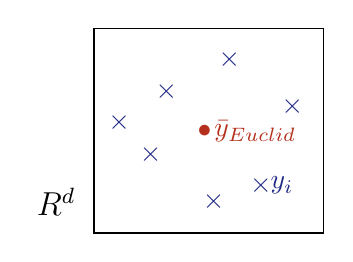
\begin{tikzpicture}[scale=2]
		\node[blue] at (0.1, 0.2) {$\times$};
		\node[blue] at (-0.1, 0.4) {$\times$};
		\node[blue] at (0.6, 0.8) {$\times$};
		\node[blue] at (0.8, 0.0) {$\times$};
		\node[blue, right] at (0.8, 0.0) {$y_i$};
		\node[blue] at (1.0, 0.5) {$\times$};
		\node[blue] at (0.2, 0.6) {$\times$};
		\node[blue] at (0.5, -0.1) {$\times$};
		\node[red] at (0.443, 0.343) {$\bullet$};
		\node[red, right] at (0.443, 0.343) {$\bar{y}_{Euclid}$};
		\draw (-0.26, -0.3) rectangle (1.2, 1);
		\node at (-0.5, -0.1) {\large $\R^d$};
	\end{tikzpicture} \hspace{2cm}
	\begin{tikzpicture}[scale=0.66]
		\shade[left color=darkWhite!90, right color=whiteGray!90] 
		(1.5,-2) to[out=15,in=170] (11.2,-1.8) node[above right] {\large $\M$} to[out=85, in=-70] (10.2,2.5) to[out=165,in=15] (1,2.2) -- cycle;
		
		\coordinate (y) at (6, 0.5);
		
		\coordinate (nu1) at (3,-0.52);
		\coordinate (nu2) at (4.15,1.4);
		\coordinate (nu3) at (8.7,-0.15);
		\coordinate (nu4) at (8.9,1.55);
		
		\coordinate (y1) at (2.45,-0.45);
		\coordinate (y2) at (4.2,1.8);
		\coordinate (y3) at (9.3,-0.5);
		\coordinate (y4) at (9.4,1.45);
		
		\draw[red, thick] (nu1) to[out=45, in=190] (y);
		\draw[red, thick] (nu2) to[out=-40, in=130] (y);
		\draw[red, thick] (nu3) to[out=130, in=-30] (y);
		\draw[red, thick] (nu4) to[out=190, in=5] (y);
		\draw[->, >=angle 60, greenTikz, thick] (y) -- node[below=2pt,pos=0.5] {$\alpha_{1,0}$} +({1.2*cos(190)}, {1.2*sin(190)});
		\draw[->, >=angle 60, greenTikz, thick] (y) -- +({1.2*cos(130)}, {1.2*sin(130)}) node[right] {$\alpha_{2,0}$};
		\draw[->, >=angle 60, greenTikz, thick] (y) -- +({1.2*cos(-30)}, {1.2*sin(-30)}) node[below] {$\alpha_{3,0}$};
		\draw[->, >=angle 60, greenTikz, thick] (y) -- +({1.2*cos(5)}, {1.2*sin(5)}) node[right] {$\alpha_{4,0}$};
		
		\node[red] at (y) {$\bullet$};
		\node[red, above right] at (y) {\large $\bar{y}$};
		
		\draw[greenTikz] (nu1) -- (y1);
		\draw[greenTikz] (nu2) -- (y2);
		\draw[greenTikz] (nu3) -- (y3);
		\draw[greenTikz] (nu4) -- (y4);
		\draw[purple] (nu1) node {$\bullet$} node[below] {\scriptsize $\Exp_{\bar{y}}(\alpha_{1,0})$};
		\draw[purple] (nu2) node {$\bullet$} node[left] {\scriptsize $\Exp_{\bar{y}}(\alpha_{2,0})$};
		\draw[purple] (nu3) node {$\bullet$} node[right] {\scriptsize $\Exp_{\bar{y}}(\alpha_{3,0})$};
		\draw[purple] (nu4) node {$\bullet$} node[above] {\scriptsize $\Exp_{\bar{y}}(\alpha_{4,0})$};
		\draw[blue] (y1) node {$\bullet$} node[left] {$y_1$};
		\draw[blue] (y2) node {$\bullet$} node[above] {$y_2$};
		\draw[blue] (y3) node {$\bullet$} node[below] {$y_3$};
		\draw[blue] (y4) node {$\bullet$} node[right] {$y_4$};
	\end{tikzpicture}
	\caption{Moyenne dans un espace euclidien (à gauche) et sur une variété (à droite).}
\end{figure}
Or comme dans les sous-section précédentes, les opérations d'addition et de multiplication par un scalaire ne sont plus nécessairement défini sur une variété. Si on veut calculer une moyenne il va falloir utiliser d'autres opérations. Pour remédier à cela on penser à une définition équivalente de la moyenne dans les espaces euclidiens comme le point qui minimise l'énergie de Fréchet.
\begin{equation}
	\bar{y}_{Euclid} = \argmin_{y_0} \sum_{i=1}^N \| y_i - y_0 \|^2
\end{equation}
On peut alors remplacer la norme par la distance géodésique sur $\M$, ce qui nous conduit à :
\begin{equation}
	\label{eq:Frechet}
	\bar{y} = \argmin_{y_0} \sum_{i=1}^N \| \Log_{y_0}(y_i) \|_{g(y_0)}^2
\end{equation}
Comme le $\Log$ n'est pas toujours facilement calculable et aussi pour éviter l'over-fitting, on utilise une version relaxé :
\begin{equation}
	\bar{y} = \argmin_{y_0} \min_{\alpha_{1,0}, ..., \alpha_{N,0}} \left[ E(y_0, \alpha_{1,0}, ..., \alpha_{N,0}) =  \sum_{i=1}^N \| \alpha_{i,0} \|_{g(y_0)}^2 + \gamma \| \Exp_{y_0}(\alpha_{i,0}) - y_i \|^2 \right]
\end{equation}
Où $\gamma$ est un facteur de relaxation. Lorsque $\gamma$ tend vers l'infini on retrouve la moyenne de Fréchet non relaxée \eqref{eq:Frechet}. L'existence de cette dernière moyenne à été prouvé. En revanche il n'y a généralement pas unicité. On remarquera aussi que le nombre de paramètre a fortement augmenté. Il ne nous reste plus qu'à réfléchir à l'optimisation.
